\documentclass[11pt]{article}
\usepackage{listings}
\usepackage[english]{babel}
\usepackage{a4}
\usepackage{latexsym}
%\usepackage[
%    colorlinks,
%    pdftitle={Design Documentation TCP Implementation},
%    pdfsubject={TCP implementation},
%    pdfauthor={Laurens Bronwasser, Martijn Vermaat}
%]{hyperref}

\pagestyle{headings}

\title{Design Documentation TCP Implementation}
\author{
    Laurens Bronwasser and Martijn Vermaat\\
    \{lmbronwa,mvermaat\}@cs.vu.nl
}
\date{31 januari 2005}

\begin{document}
\maketitle


\lstset{
  numbers=none,
  basicstyle=\small,
  frame=tb,
  language=C,
  captionpos=b
}


\section{High-level design}

For the implementation for the TCP library, we decided to follow a three-tier
design. The three tiers of our implementation are the following:

\begin{enumerate}
\item the connection-ori\"ented tier
\item the state tier
\item the connection-less tier
\end{enumerate}

The connection-ori\"ented tier provides a TCP interface to the application
layer, whereas the connection-less tier deals only with sending and
receiving TCP packets and works directly on the IP layer interface.

The middle layer in our implementation will be the state tier. This tier
will have to bridge the gap between a connection-less environment and a
connection-ori\"ented environment, and therefore has to maintain a state.

\paragraph{}

Calling of procedures happens only within one tier, or from one tier to
the tier directly beneeth it. This is good programming practice, as it makes
debugging and reuse of code more feasable.


\section{Provided functions}

We will now discuss the functions provided by our TCP implementation, how they
can be called, and what there semantics are. These functions are all declared in
the \lstinline|tcp.h| header file.


\subsection{\lstinline{tcp_socket}}

Initializes TCP state.

\begin{lstlisting}
int tcp_socket(void);
\end{lstlisting}

\paragraph{Return value}

Returns 0 on success, -1 on failure.

\paragraph{Description}

Before calling any other function provided by the TCP library,
\lstinline|tcp_socket| must be called. If it is called at any later time, it
will reset the TCP state and close any open connection.


\subsection{\lstinline{tcp_connect}}

Connects to a server.

\begin{lstlisting}
int tcp_connect(ipaddr_t dst, int port);
\end{lstlisting}

\paragraph{Return value}

Returns 0 on success, -1 on failure.

\paragraph{Description}

This function tries to connect to a server on address \lstinline|dst| at port
\lstinline|port|. When TCP is not in a closed state, \lstinline|tcp_connect|
fails. If you want to make a new connection while not in a closed state, call
\lstinline|tcp_socket| first.


\subsection{\lstinline{tcp_listen}}

Wait for an incomming connection to establish.

\begin{lstlisting}
int tcp_listen(int port, ipaddr_t *src);
\end{lstlisting}

\paragraph{Return value}

Returns 0 on success, -1 on failure.

\paragraph{Description}

This is a blocking function. It listens on port \lstinline|port| for an
incomming connection. Upon successful establising of the connection,
\lstinline|tcp_listen| succeeds. When TCP is not in a closed state,
\lstinline|tcp_listen| fails. If you want to listen for a new incomming
connection while not in a closed state, call \lstinline|tcp_socket| first.


\subsection{\lstinline{tcp_close}}

Close active connection.

\begin{lstlisting}
int tcp_close(void);
\end{lstlisting}

\paragraph{Return value}

Returns 0 on success, -1 on failure.

\paragraph{Description}

This function tries to close the active connection. It always succeeds, except
when there is not active connection; then it fails.


\subsection{\lstinline{tcp_write}}

Write data to other side.

\begin{lstlisting}
int tcp_write(const char *buf, int len);
\end{lstlisting}

\paragraph{Return value}

Returns the number of bytes written, or -1 on failure.

\paragraph{Description}

This function 


\subsection{\lstinline{tcp_read}}

Read data from other side.

\begin{lstlisting}
int tcp_read(char *buf, int maxlen);
\end{lstlisting}

\paragraph{Return value}

Returns the number of bytes read, or -1 on failure.

\paragraph{Description}

This is a blocking function. It reads data from the other side, until
\lstinline|maxlen| a maximum of bytes are read. The read data is copied to
\lstinline|buf|. If the other side has closed the connection and there is no
more data, \lstinline|tcp_read| returns 0.

When there is no active connection, \lstinline|tcp_read| fails.


\subsection{Some additional notes}

\paragraph{Closing connections}

Closing a connection in TCP has a special meaning. It does not just mean you
will stop communicating, but 

\paragraph{Signals}




\section{Design decisions}


\paragraph{Buffer for incoming data}
    The buffer for incoming data is bigger than the maximum payload of a tcp
    packet. This is necessary because new data might come in while for example 
    \lstinline|tcp_write()| is polling for ack's. These data must be stored in the 
    buffer; 
    there is no way we can deliver it to the user.
    The buffer is circular because this prevents shoving of data to the begin of 
    the buffer to fill the gaps. 
    The state of the buffer is comprised in a variable that points to the 
    current start of the buffer, a variable that indicates the amount of data in 
    the buffer and of course the buffer itself.    

\paragraph{Pushing of incoming data}
    We don't assume that every incoming packet has the PSH flag set, eventhough 
    the assignment prescribes to set PSH on all outbound packets. That we do
    check the PHS flag means 
    that if it is set, \lstinline|tcp_read()| delivers is the data immediately.
    Only if there is no data to be pushed, \lstinline|tcp_read()| keeps on polling 
    ip for 
    more data until the amount of data specified by the user is received.
    
    \lstinline|tcp_read()| might return less (if the \lstinline|PSH| flag is set), but 
    the \lstinline|PSH| flag 
    will never cause \lstinline|tcp_read()| to return more 
    data than indicated by the users parameter.
    
    To keep track of the number of bytes that need to be pushed, a variable is 
    added to the tcb: \lstinline|rcvd_data_push|.

\paragraph{Acknowledgements}
    If data comes in tcp has never seen before (i.e. fresh data), an 
    acknowledgement is send
    immediately by \lstinline|handle_data()|. In real tcp implementations sending of
     ack's 
    should be postponed until the data is actually delivered to the user, 
    but since the assignment prescribes to use a window of size 1, we have to 
    acknowledge each packet instantly.

\paragraph{Connection establishment}
    After the first \lstinline|syn| is sent, 
    the state transits to \lstinline|SYN_SENT| 
    and we wait for the \lstinline|syn+ack| response. In this state, only 
    \lstinline|syn+ack| packets will be accepted. If a packet arrives that carries an
    acknowledgement, but no \lstinline|syn|, this packet will be rejected.
    Also, a packet with a \lstinline|syn| must contain an ack. 
    If a \lstinline|syn+ack| does not arrive within the specified 
    \lstinline|round trip transmition time| the state will be altered to 
    \lstinline|CLOSED|. Thereafter the \lstinline|syn| is automatically 
    resend, which causes the state to go to \lstinline|SYN_SENT| again.
    
    
\paragraph{State transitions}
    The \lstinline|declare_event()| procedure performs all necessary state 
    transitions, based on the event that is passed as a parameter to this 
    procedure. For example, 
    is the state is \lstinline|S_LISTEN| and a \lstinline|syn| is received, 
    \lstinline|E_SYN_RECEIVED| is passed to \lstinline|declare_event()|. The state will 
    then be altered to \lstinline|S_SYN_RECEIVED|. 
    In this way, \lstinline|declare_event()| directly implements the state 
    transition diagrams shown in appendix \ref{sec:A}.
    
    There is a trade-off here between straightforward source code and source 
    code that has some build in bug-detection, which are both preferable. If we 
    had chosen for straightforward code, we had \lstinline|declare_event()| swallow
    every event that takes place. For example \lstinline|handle_ack()| would then 
    consist of only one line: 
    \lstinline|if (ack_flag) {declare_event(E_ACK_RECEIVED)}|. Then we leave it to 
    \lstinline|declare_event| to decide if a state transition is necessary.
    On the other hand, if
    some unexpected event happens, we wouldn't notice, because 
    \lstinline|declare_event()| gracefully discards the event, without any warning.
    
    To make it easier to detect unexpected events (caused by a bug), we decided 
    to make \lstinline|declare_event| accept only the events that are defined in the
    state transition diagram. On all other events it starts to yell (on the 
    screen). The consequence is that some code is a little bit more complex, 
    because we can't just say \lstinline|declare_event(E_ACK_RECEIVED)|
    on every incoming ack. We first have to check whether this ack event may 
    declared for a state transition.
    
    
\paragraph{Wrapping sequence numbers}
    The sequence number and ack numbers have to be wrapped after hitting the 
    highest value that can be represented with 32 bits. This wrapping occurs 
    automatically if unsigned 32 bit variables are used. The issue is that 
    this implementation will only work when \lstinline|unsigned long| is 
    exactly 32 bits long.
    
    Of course, we still have to be aware of wrapping sequence numbers when we do
    comparisons involving sequence numbers or acknowledgement numbers.



\subsection{TCP Control Block}


The \lstinline|tcb| (TCP Control Block) contains all information on the
current state. This includes client and host addresses and ports, buffer
data, packet sequence number, etcetera.


\paragraph{}


\subsection{Connection-less tier}

The only two procedures in this tier are \lstinline|send_tcp_packet()| and
\lstinline|recv_tcp_packet()|.

\paragraph{Procedure recv\_tcp\_packet()}
This procedure calls \lstinline|ip\_receive()| only once. If a packet is corrupted,
or if it is no tcp packet at all, \lstinline|recv\_tcp\_packet| returns -1.
That it does not loop to wait for a valid packet, is because this might take 
forever. The looping is taken care of by \lstinline|tcp\_read()|, which checks if the alarm 
went of on every cycle.

\appendix

\section{State transition diagrams} \label{sec:A}

\paragraph
The three way handshake diagram shows the states we use in our TCP 
implementation. A capital label denotes a call to TCP by the application. 
The other labels refer to events that are caused by TCP itself, for example 
incoming packets or timers that go off. \lstinline|partner_dead| means that 
after resending a packet 10 times, the other party is considered to be retired.



\begin{figure}
\begin{center}
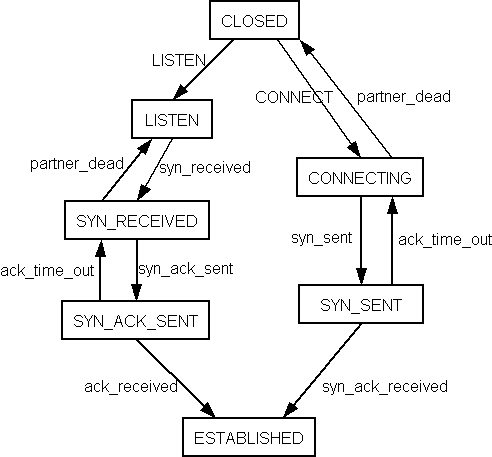
\includegraphics{images/handshake.png}
\end{center}
\caption{Three way Handshake}
\label{figuur:handshake}
\end{figure}

\begin{figure}
\begin{center}
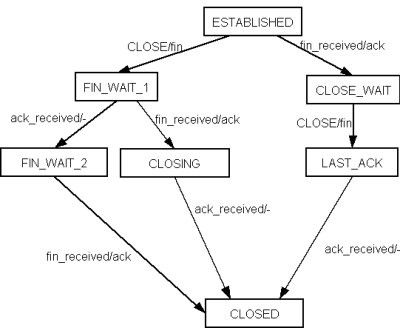
\includegraphics{images/termination.png}
\end{center}
\caption{Connection termination}
\label{figuur:termination}
\end{figure}


\end{document}

